\frame{
  \frametitle{Interval Tree}
  \begin{itemize}
    \item Given a set of ranges, query for the intervals that contain a specified point in $O(\log n + $number of crossing intervals$)$.

    \medskip 

    \item Each node stores all intervals crossing a certain point.
  \end{itemize}
  \begin{center}
  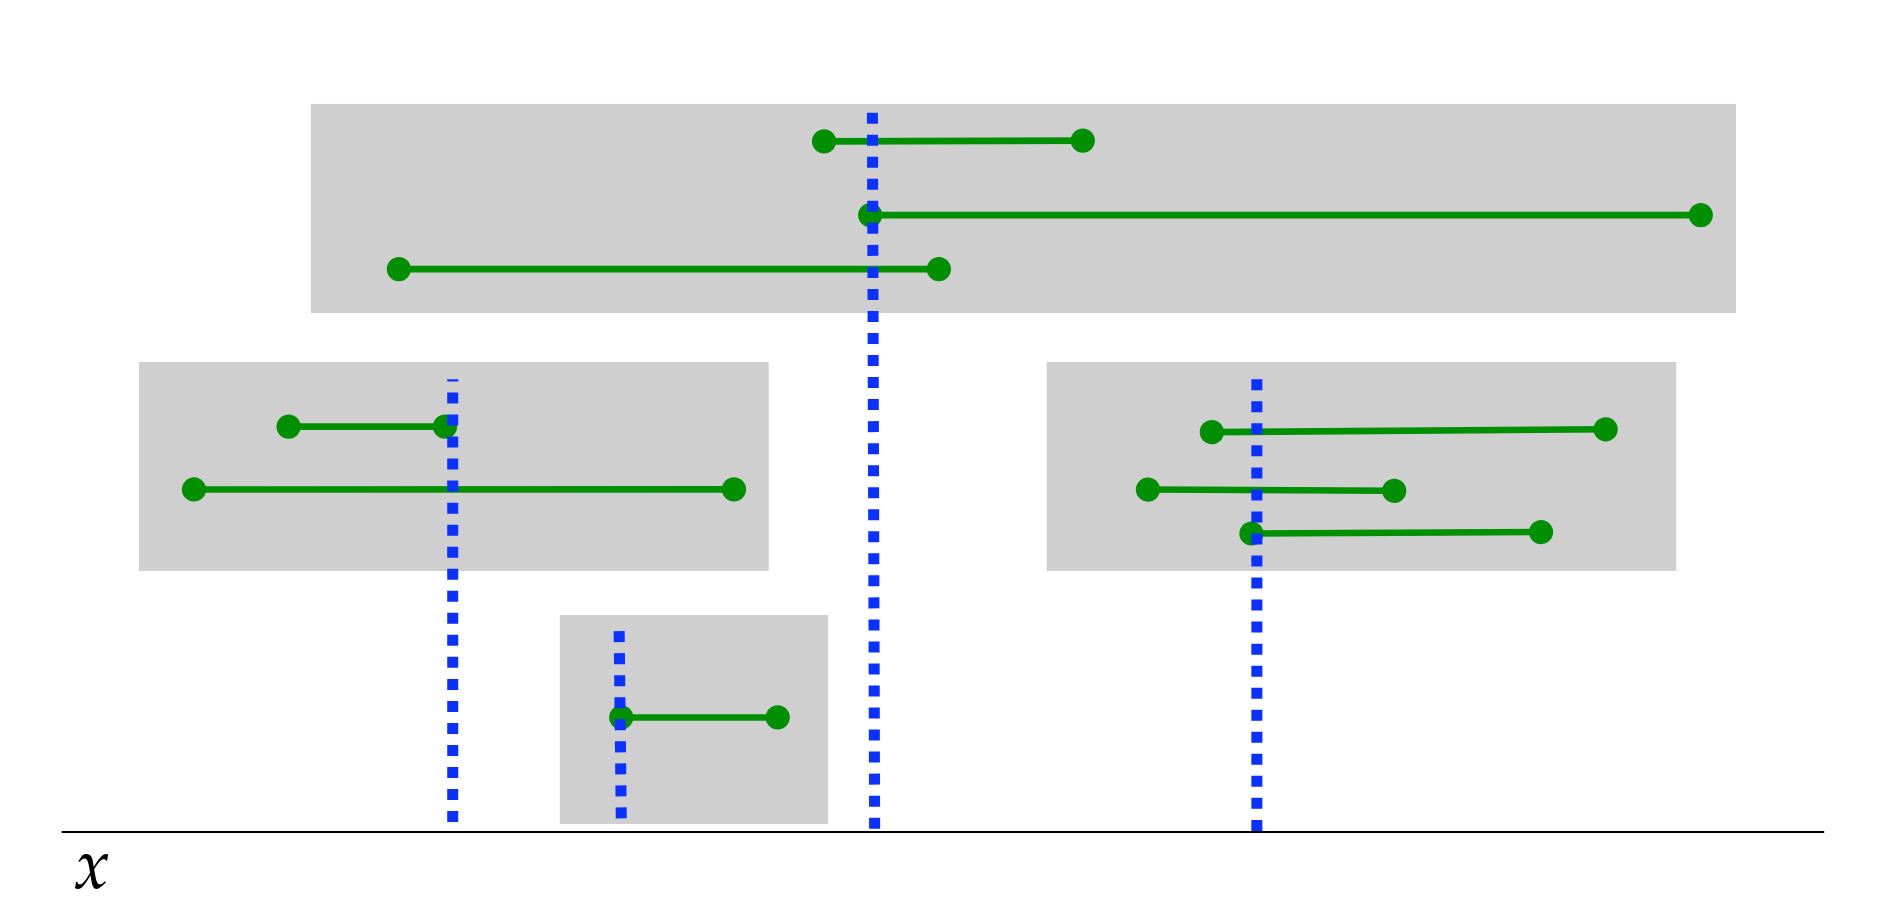
\includegraphics[scale=0.15]{slides/alphabet_trees/interval_tree.png}
  
  \tiny{https://www.cs.cmu.edu/~ckingsf/bioinfo-lectures/intervaltrees.pdf}
  \end{center}
}